\chapter{FUTURE WORK}
\label{chap:satfx}
\label{chap:future_work}


\section{Satellite Image Forecasts}
\label{sec:satellite_fx}

\Cref{chap:satoi} and \cref{app:satoi} present a way in which a
nowcast of irradiance can be improved using data assimilation
techniques.
Naturally, we want to extend this nowcast into a proper forecast
initially using the technique of cloud motion vectors that produced
forecasts in \cref{chap:network} and \cref{app:network}.
More complicated dynamics other than advection such as cloud formation
and dissipation may be incorporated.
Eventually, a full numerical weather model may be required to capture
the dynamics of the system with the desired accuracy.


With a forecast model, it is natural to extend optimal interpolation
to the well known Kalman filter where a forecast of the state is
produced and constantly updated with new information.
This has the added benefit of retaining information from all previous
steps.
Errors will be present in an estimation of the cloud velocity field,
thus we will use an ensemble Kalman filter with an ensemble of
velocity fields.
An additional challenge will be integrating two types of observations
into the state of the system: new observations from ground sensors and
new satellite images.


In addition to introducing the forecast model and Kalman filter, we
will also explore extending the area of analysis and the number of
observations used.
\Cref{fig:allsensors} shows the locations of roughly 300 sensors that
may provide useful information to this data assimilation problem.
Some sensors such as the SURFRAD and NREL MIDC sites are regularly
maintained, calibrated, and report high resolution data.
Other sites such as those in the RAWS network provide hourly
irradiance values and may lack routine maintenance.

\begin{figure}[h]
\centering
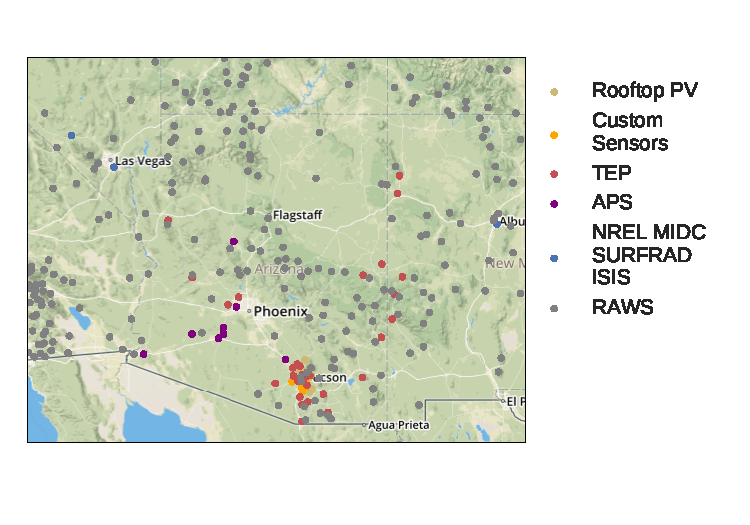
\includegraphics[width=\textwidth]{figs/azmap.pdf}
\vspace{-3em}
\caption[Map of all available irradiance sensors]{Map of all currently
available irradiance sensors near Arizona. These sensors come from a
number of networks with varying quality and time resolutions.}
\label{fig:allsensors}
\end{figure}

With the launch of the GOES-16 geostationary satellite, a number of
groups are developing products and algorithms that make use of the new
Advanced Baseline Imager (ABI) and will provide better background
state estimates.
The new ABI will image the continental US every five minutes with 16
spectral bands and resolutions as high as 0.5 km for the 0.64 $\mu$m
visible band.
Pictures of a comparison of the new GOES-16 and the current GOES-13
visible images in \cref{fig:goes_comp} and of a detailed image over
California in \cref{fig:goes_cal} show the impressive capabilities of
the instrument.

\begin{figure}[t]
\centering
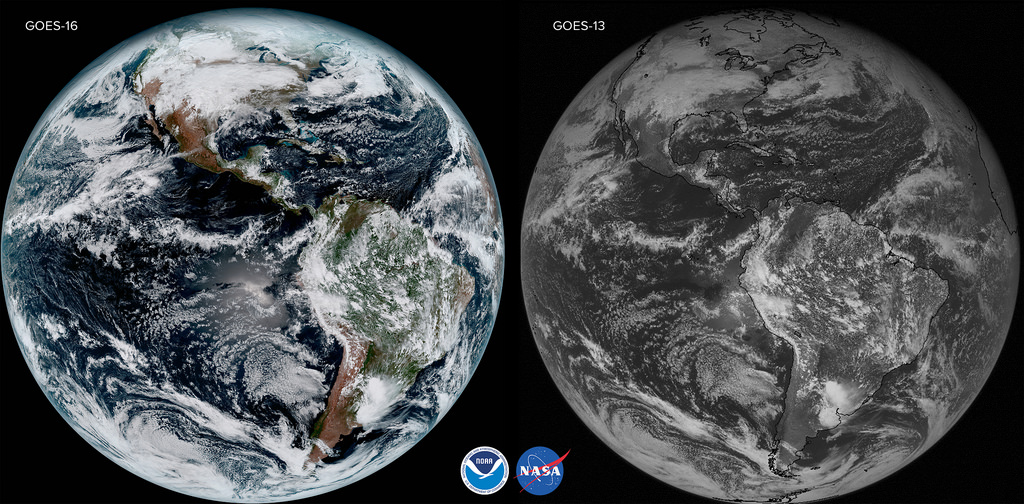
\includegraphics[width=\textwidth]{figs/goes_comp.jpg}
\caption[Comparison of visible images from the current and future
GOES]{A comparison of visible images created from the visible channels
of the new GOES-16 satellite and the previous generation
GOES-13. GOES-13 has only a single visible channel while GOES-16 has
three. Image courtesy of NOAA.}
\label{fig:goes_comp}
\end{figure}

\begin{figure}[h]
\centering
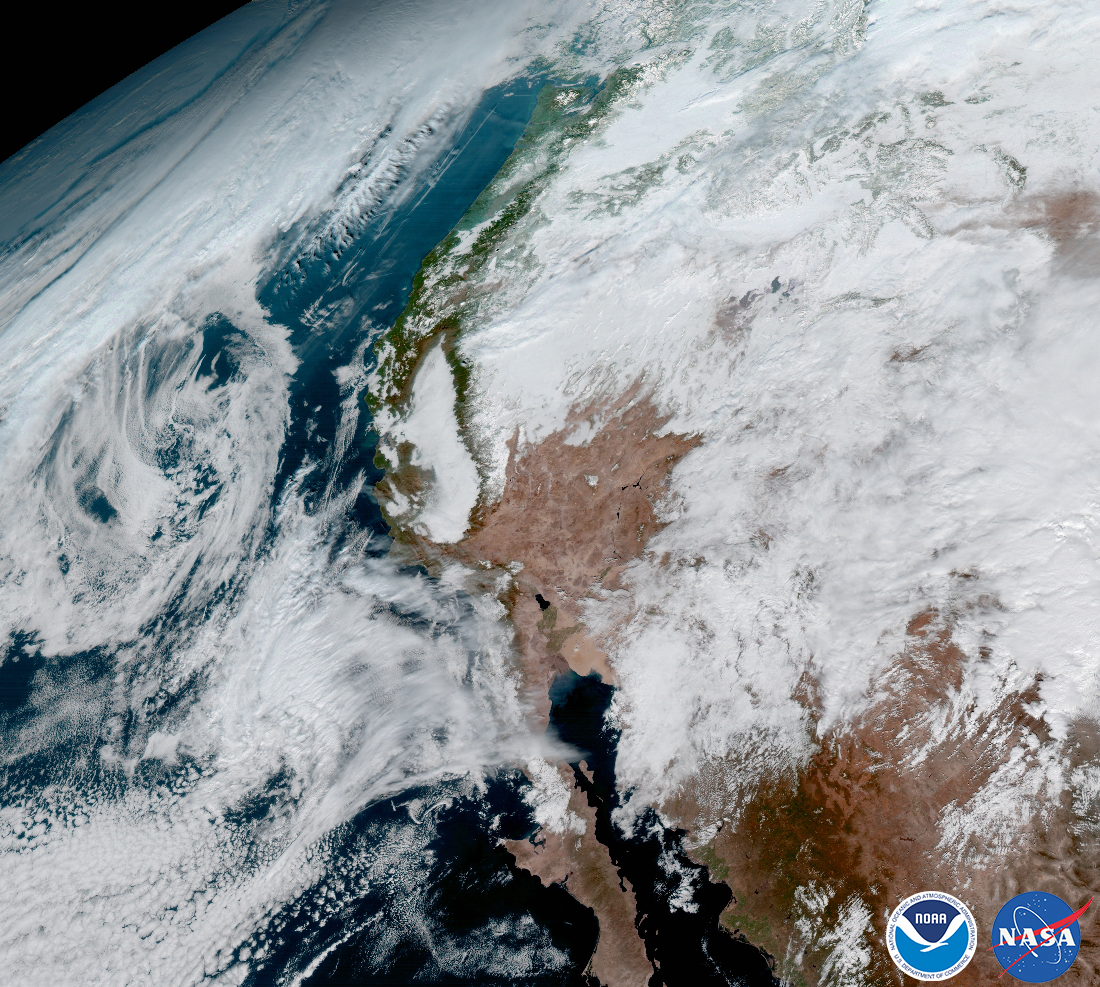
\includegraphics[width=0.8\textwidth]{figs/goes_cal.jpg}
\caption[An visible image of the western US from GOES-16]{A visible
image of the western US from the new GOES-16 satellite. The improved
resolution and spectral bands will improve satellite derived
irradiance estimates compared to the current generation of
satellite. Image courtesy of NOAA.}
\label{fig:goes_cal}
\end{figure}

A forecast regenerated every 5 minutes for 5 minutes to 6 hours in
advance covering a $300 \times 300$ km area over the state of Arizona
with 0.5 km resolution satellite estimates and 300 sensors from a 50
member (or larger) ensemble is a computationally daunting task.
Initial research into the local ensemble transform Kalman filter to
reduce the computational demands is promising \citep{Hunt2007}.
Still, producing these forecasts operationally will likely require use
of a high performance computing cluster and specialized compute
hardware such as GPUs or coprocessors.

\section{Cloud Data Assimilation in WRF}

Forecasts produced by the Weather Research and Forecasting (WRF)
numerical weather model at the University of Arizona tend to lack
clouds.
Given the large area coverage that satellite images provide, it is
natural to consider assimilating clouds from satellite images into the
WRF model.
This is a nontrivial task because the model does not produce clouds
directly and the errors in cloud properties derived from satellite
images can be difficult to estimate.
Previous work has had some success by comparing the WRF cloud fields
and satellite imagery to modify the water vapor variable in WRF
\citep{Mathiesen2013}.
This is a good starting point for future work, but ideally other
properties of the cloud such as the ice and water content, depth,
etc.\ would be accounted for.

\section{Ensemble WRF Forecasting}

An ensemble of WRF forecasts, similar to the ensemble of satellite
forecasts discussed in \cref{sec:satellite_fx}, may produce better
forecasts by spanning more of the solution space.
This is regularly done at operation forecasting centers.
Currently, UA-WRF is run about six times a day with different initial
conditions based on the 0Z, 6Z, and 12Z GFS and NAM forecasts.
This produces a multi-physics, time-lagged ensemble.
Additional ensemble members can be produced by varying the various
parameterizations in the model such as the microphysics and planetary
boundary layer schemes.
This will require study of model performance differences with
different schemes to ensure ensemble members have a reasonable spread
to avoid wasting computation on members that always produce the same
forecast.

\section{Intelligent Forecast Fusion}

As mentioned in \cref{chap:intro}, one eventual goal is to combine
different types of forecasts taking into account their relative
accuracies at different time horizons into one unified forecast.
This unified forecast would predict future vales from one minute in
the future out to seven days combining persistence, network,
satellite, and numerical weather forecasts.
The main challenges to achieving this goal are deciding the time
horizon where one forecast ends and another begins and ensuring the
forecast is consistent over this transition.

One technique to produce this fused forecast is compute a weighted sum
of all the forecasts where the weights are dependent on the forecast
horizon.
Then the challenge becomes choosing the weights.
Ideally, these weights would be based on the errors in the forecasts
at different time horizons.
The errors can be calculated using a year of past data and forecasts,
but the errors will vary depending on the weather and season.
One way to account for this may be to establish categories such as
clear days, days with high thin clouds, etc.\ and compute errors for
each category.
Then, one just determines the category for the day and applies the
weights based on the category.
In some sense, this is an analog method.
Another option may be to use machine learning techniques to determine
the weights between forecasts.

%%% Local Variables:
%%% mode: latex
%%% TeX-master: "dissertation"
%%% End:
